\documentclass[a4paper,10pt]{article}

\usepackage[utf8]{inputenc}
\usepackage[margin=1in]{geometry}
\usepackage[spanish,es-noquoting]{babel}
\usepackage{fancyhdr}
\usepackage{float}
\usepackage{incgraph,tikz}
\usepackage{hyperref}
\usepackage{listings}

%Code
\lstset{ %
basicstyle=\small,       % the size of the fonts that are used for the code
numbers=left,                   % where to put the line-numbers
numberstyle=\footnotesize,      % the size of the fonts that are used for the line-numbers
stepnumber=1,                   % the step between two line-numbers. If it is 1 each line will be numbered
numbersep=5pt,                  % how far the line-numbers are from the code
backgroundcolor=\color{white},  % choose the background color. You must add \usepackage{color}
showspaces=false,               % show spaces adding particular underscores
showstringspaces=false,         % underline spaces within strings
showtabs=false,                 % show tabs within strings adding particular underscores
frame=single,           % adds a frame around the code
tabsize=4,          % sets default tabsize to N spaces
captionpos=b,           % sets the caption-position to bottom
breaklines=true,        % sets automatic line breaking
breakatwhitespace=false,    % sets if automatic breaks should only happen at whitespace
escapeinside={\%*}{*)}          % if you want to add a comment within your code
}

%Captions
\renewcommand{\lstlistingname}{Código}
\renewcommand\spanishtablename{Tabla}
\renewcommand{\figurename}{Gráfico}

\pagestyle{fancy}

\renewcommand{\baselinestretch}{1.5} 

\makeatother

\title{Bosque de Obstáculos}
\author{Badi Leonel, Buchhalter Nicolás Demián y Meola Franco Román}
\lhead{Bosque de Obstáculos}
\rhead{Trabajo Práctico Final}

\begin{document}

\maketitle

\pagebreak

\tableofcontents

\newpage

\section{Introducción}

En el presente trabajo se detallan los fundamentos, la implementación y los resultados obtenidos de la simulación del trayecto de un peatón equipado con un mecanismo de navegación que viaja desde un punto inicial a uno final con el objetivo de  evitar colisiones con los obstáculos fijos presentes en la escena. Para la simulación se utiliza una implementación propia del \textit{Contractile Particle Model} y no se utilizaron plataformas de simulación peatonal.

Los fundamentos están inspirados en la temática \textit{Steering Behavior}, propuesto por Mat Buckland en su libro \textit{Programming Game Ai by Example}, así como también en los conocimientos de método de búsqueda informados.

El objetivo principal del presente trabajo consiste en crear una heurística que permita ajustar dinámicamente el ángulo del versor de la velocidad deseada en función de las posiciones de los ángulos. Para lograrlo, se recurre una versión modificada del método de búsqueda informado A* que utiliza la heurística distancia real al objetivo. Cabe destacar que la búsqueda de la ruta se realiza antes de la simulación, ya que todos los obstáculos a evitar son fijos. Por último, se modifica el \textit{Contractile Particle Model} para evitar colisiones en el transcurso la simulación.

\section{Fundamentos}

En esta sección se detallan todos los fundamentos teóricos que sustentan el presente trabajo así como también los parámetros fijos que se definieron para todas las pruebas realizadas.

\subsection{Escena}

A continuación se listan los parámetros que permanecen fijos en todas las pruebas que se explicarán en el análisis de resultados.
En cuanto al agente del \textit{Contractile Particle Model} que recorrerá la escena y deberá inteligentemente esquivar los obstáculos fijos, los parámetros son los siguientes:
\begin{itemize}
	\item $r_{0} = 0.25m$
	\item $r_{min} = 0.15m$
	\item $r_{max} = 0.32m$
	\item $v_{d}^{max} = 1.55 \frac{m}{s}$
\end{itemize}
donde $r_{0}$ es el radio inicial del agente y el cual puede variar en el intervalo $[ r_{min} , r_{max} ]$ y $v_{d}^{max}$ es la velocidad deseada del agente.

Se definieron además los valores de los siguientes parámetros fijos del modelo
\begin{itemize}
		\item $\tau = 0.5s$
		\item $\beta = 0.9$
\end{itemize}
donde $\tau$ se utiliza para el cálculo de la evolución temporal del radio del agente y $\beta$ para el cálculo de $|v_{d}|$. 

Se decidió utilizar una habitación cuadrada de $25m$ de lado, donde se colocan aleatoriamente 300 obstáculos fijos, todos del mismo radio $r_{obstaculo} = r_{0}$. Como se puede ver en la Figura \ref{fig:scene}, la posición inicial del agente está en la esquina inferior izquierda y la destino está en la esquina superior derecha. Se prevee no colocar obstáculos muy cerca de la posición inicial y final del agente. Sin embargo, no se prohíbe la superposición de obstáculos, de forma de permitir la formación de paredes de obstáculos.

\begin{figure}[H]
	\centering
    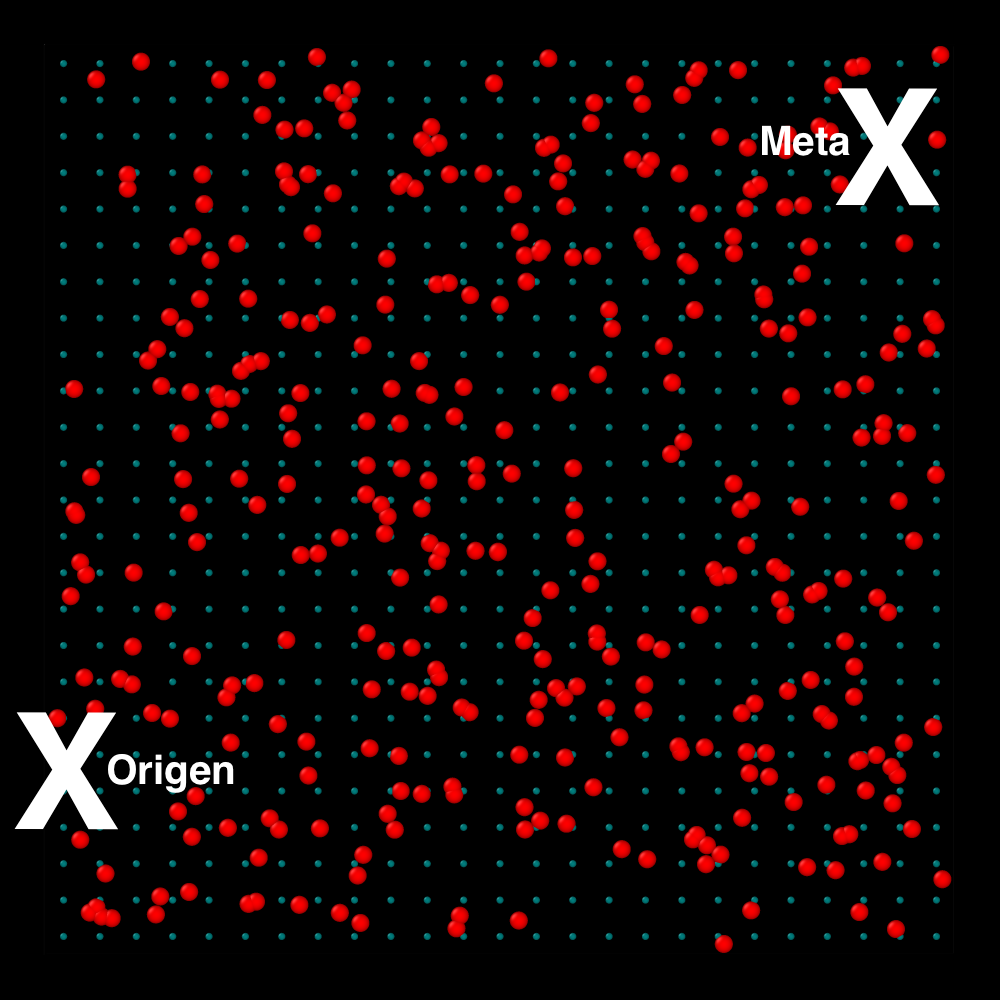
\includegraphics[width=0.75\textwidth]{images/scene.png}
    \caption{Ejemplo de escena con 300 obstáculos fijos distribuidos aleatoriamente. La posición inicial del agente (origen) se encuentra en la esquina inferior izquierda y la posición final del agente (meta) se encuentra en la esquina superior derecha.}
    \label{fig:scene}
\end{figure}

\subsection{Métodos de Búsqueda Informados}

El objetivo de un método de búsqueda es encontrar un camino entre el estado inicial y el estado final. Los métodos de búsqueda desinformados sólo utilizan el costo de búsqueda $g(n)$, de forma que se obtiene una búsqueda a ciegas y resulta muy ineficiente. Por lo tanto, es necesario agregar valores que estimen cuánto falta para alcanzar el objetivo. 

A estos métodos de búsqueda se los denomina informados y forman parte de la familia de algoritmos \textit{Best First} (el primer nodo a explorar es el de menor costo). Se define así una heurística $h(n)$ como el costo estimado de la ruta más barata que une el estado del nodo $n$ con un estado meta. 

El método de búsqueda informado utilizará la función de mínimo costo de ruta $f(n) = g(n) + h(n)$ donde para la Figura \ref{fig:graph}
	\begin{itemize}
		\item $g(n):$ es el costo de la ruta que va del nodo inicial hasta el nodo $n$
		\item $h(n):$ estimación del mínimo costo de ruta que va de $n$ al nodo objetivo
		\item $f(n):$ costo estimado de la solución más barata que pasa por $n$
	\end{itemize}
	
\begin{figure}[H]
	\centering
    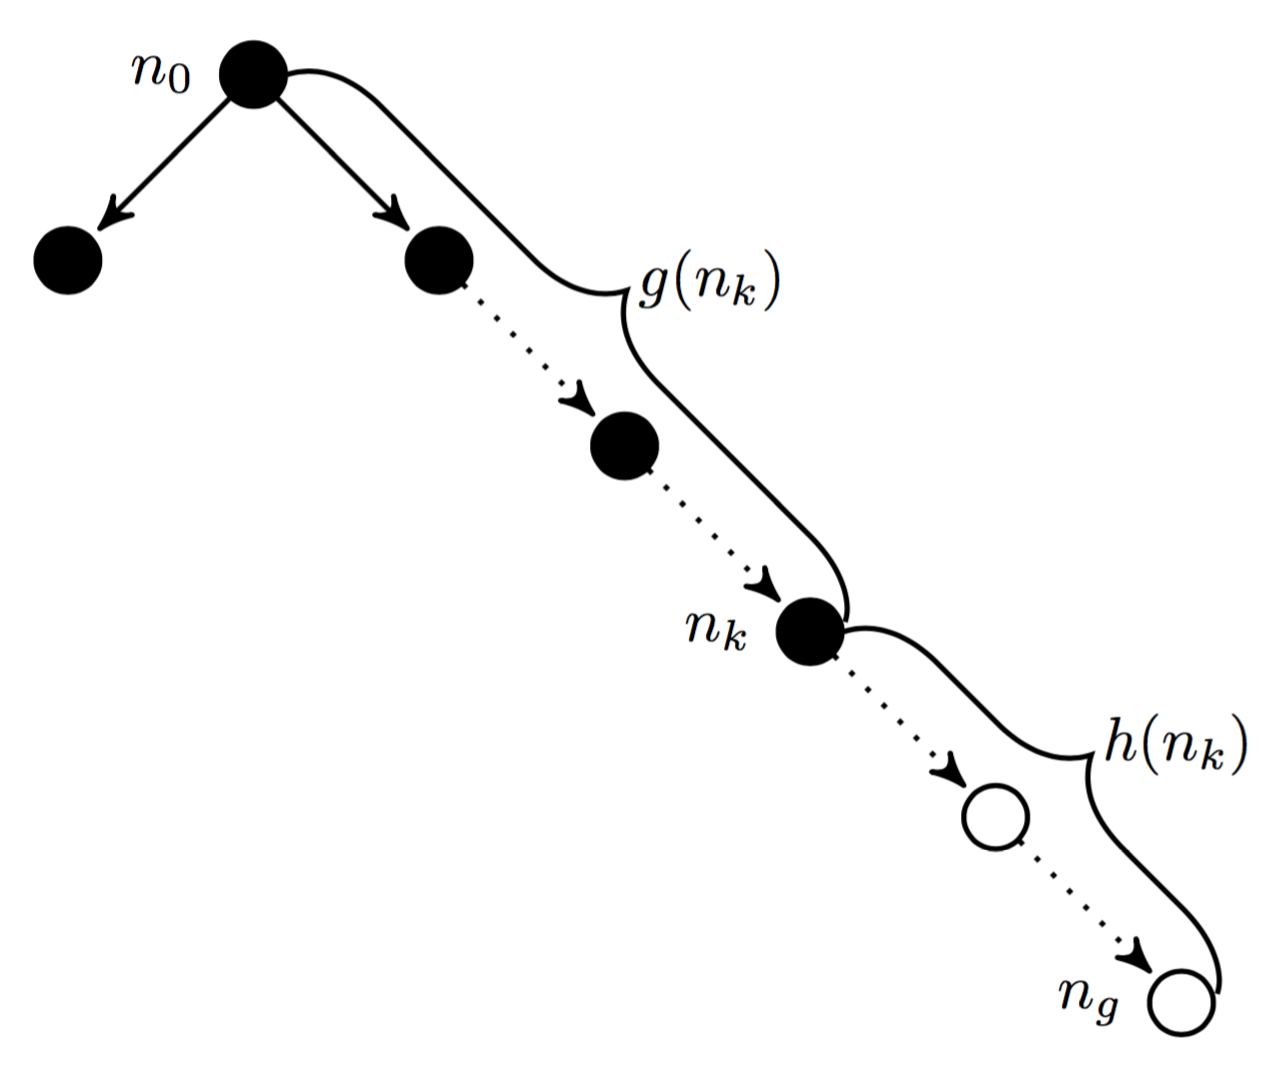
\includegraphics[width=0.50\textwidth]{images/graph.png}
    \caption{Diagrama de aplicación del mínimo costo de ruta para un árbol de búsqueda.}
    \label{fig:graph}
\end{figure}
	
Habiendo definido la función $f$, se explica en una sucesión ordenada de pasos el algoritmo de búsqueda informado A*:
\begin{enumerate}
\item Crear un árbol de búsqueda, $T_{r}$, que sólo esté formado por el nodo inicial $n_{0}$. Insertar $n{0}$ en la estructura FRONTERA.
\item Crear el conjunto EXPLORADOS, inicialmente vacío.
\item Si FRONTERA está vacía, el algoritmo termina con falla.
\item Extraer el primer nodo de FRONTERA e insertarlo en EXPLORADOS. Llamar a este nodo $n$.
\item Si $n$ es el nodo objetivo, salir del algoritmo y devolver la solución, que está formada por el camino definido por los arcos que llevan de $n$ a $n_{0}$ en el árbol $T_{r}$.
\item Expandir el nodo $n$ y generar el conjunto de nodos sucesores $M$. Incorporar los elementos de $M$ como sucesores de $n$ en el árbol $T{r}$, creando los arcos correspondientes entre $n$ y cada uno de los nodos de $M$.
\item \textbf{Reordenar FRONTERA de forma que primero estén los nodos de menor $f$}.
\item Ir al paso 3.
\end{enumerate}

El comportamiento de A* está directamente relacionado con la heurística $h$ utilizada. Es necesario mencionar que una heurística es admisible si nunca sobreestima el costo real. De esta forma, si $h$ es admisible entonces $f(n)$ nunca sobreestima el costo real de la mejor solución que pasa por $n$. Sólo con $h$ admisible, el algoritmo A* es completo y admisible, de forma que se garantiza siempre encontrar el camino óptimo al objetivo, si es que existe uno.

En resumen, A* actúa sobre un grafo donde el objetivo es encontrar el camino de costo mínimo, eligiendo para expandir siempre el nodo de menor $f$. El problema es que al actuar sobre un grafo, el espacio de búsqueda debe ser discreto. Es por eso que se requiere hacer una adaptación de la escena para poder discretizar posiciones de la habitación.

\section{Implementación}

En esta sección se detallan las modificaciones que se realizaron al método de búsqueda informado y al modelo de dinámica peatonal para obtener mejores resultados en la simulación propuesta.

\subsection{Adaptación del método de búsqueda}

El primer problema encontrado consiste en implementar A* en un sistema continuo: es necesaria la discretización del sistema. Para resolver este problema se definió el concepto de \textit{waypoint}.

Un \textit{waypoint} es un punto $(x,y)$ en la escena por donde el agente podrá desplazarse. Estos serán los \textbf{nodos} por donde iterará el método de búsqueda. En el caso de este trabajo, el espacio a simular cubre toda la escena, pero en casos más complejos este sistema es flexible para tomar la forma que se desea. Por ejemplo se pueden definir \textit{waypoints} sólo por ciertas áreas de un plano que son transitables. Cabe aclarar que en este modelo, los \textit{waypoints} pueden estar colocados en cualquier posición de la escena. De esta manera se pueden colocar a diferentes distancias entre sí, siendo más potente que una simple grilla de casilleros.

Se decidió armar una grilla de \textit{waypoints} sobre la habitación donde  los \textit{waypoints} están separados unos de otros por una distancia $W_{d}$. Otro de los parámetros que se pueden variar en el modelo es el grado de conectividad entre los \textit{waypoints}. Este parámetro se denomina ventana y representa el número de vecinos aledaños del \textit{waypoint}. Para un \textit{waypoint}, la ventana es siempre cuadrada y se llama $W_{v}$ a la longitud del lado de la ventana. De esta forma, si $W_{v} = 3$ la ventana contiene a los 8 vecinos aledaños. Si $W_{v} = 5$, la ventana contiene a los 24 vecinos. 

El algoritmo de \textit{pathfinding} de la implementación consiste en una modificación de A* donde el grafo a recorrer es el formado por los \textit{waypoints} y sus conexiones. El conjunto de vecinos de la ventana del nodo $n$ constituye a los nodos sucesores del mismo. El objetivo es obtener una lista de \textit{waypoints} por donde el agente tiene que transitar desde el nodo inicial hasta alcanzar el nodo meta. La lista de \textit{waypoints} obtenida se define como un conjunto de sub-objetivos que tiene que ir recorriendo el agente. Así, para cierto momento dado, el versor velocidad del agente tiene como dirección a la línea que se forma entre la posición actual del agente y el primer sub-objetivo.


\subsection{Definición de heurística}

La heurística $h(n)$ es la distancia real que se tiene al objetivo (distancia en línea recta al nodo meta). Esta heurística es admisible ya que no sobreestima la solución y el costo es la distancia que ya se recorrió. De esta forma, A* será completo y admisible, y siempre encontrará el camino óptimo al objetivo si es que existe uno.

\subsection{Búsqueda limitada en profundidad}

Una modificación implementada fue la limitación en profundidad de la búsqueda de la solución óptima. El árbol de búsqueda tiene un máximo de profundidad $L$ y en el borde del límite se encuentra un nodo meta sub-óptimo. Una vez alcanzado el sub-óptimo, se reinicia la búsqueda desde allí.

\subsection{Detección de colisiones}

Otra de las modificaciones al algoritmo original es la detección de posibles colisiones en caminos. Para detectarlo se genera un \textit{raycast}, es decir un rayo en línea recta desde un \textit{waypoint} origen hacia otro waypoint \textit{destino}. Si el trayecto del \textit{raycast} impacta sobre un obstáculo, entonces ese camino es descartado del árbol de búsqueda. Así se evitan muchas colisiones innecesarias y caminos sin salida.

\subsection{Prevención de colisiones}

Los \textit{steering behaviors} son comportamientos que se le pueden aplicar al agente para que se comporte de una manera determinada. Con cada \textit{steering behavior} se obtiene un vector velocidad normalizado, que luego sumado, resulta en un vector velocidad que representa el comportamiento del agente en ese instante.

El objetivo entonces es evitar los choques del agente con obstáculos que tiene en sus inmediaciones. Así, utilizando una partícula de radio $r_{p} = 1.1 r$ se calculan todos los posibles solapamientos con obstáculos. Para cada solapamiento detectado se genera un versor director en dirección contraria a la del agente, para así evitar este obstáculo. Al final, todos los versores se suman y se obtiene un versor sumarizado que representa la dirección a transitar para no colisionar con los obstáculos.

%\begin{lstlisting}[language=Java, caption = Algoritmo de simulación]
%public void simulate(double t, double dt, int k){
%	writeFrame(0);
%	int framesWrited = 1;
%	double totalTimeSimulated = 0;
%	moveSystem(dt);
%	totalTimeSimulated += dt;
%	while(totalTimeSimulated < t){
%		for(int i = 0; i < k; i++){
%			moveSystem(dt);
%			totalTimeSimulated += dt;
%		}
%		writeFrame(framesWrited++);
%	}
%}
%\end{lstlisting}

\section{Resultados}

Lorem ipsum dolor sit amet.

\section{Conclusiones}

Lorem ipsum dolor sit amet.

\end{document}
